\section{Experimental Detail}
\label{app:evaluation-detail}

The following appendix preserves the v3.3 natural-corpus, reference-pool,
runtime and capability tables and by-invariant plots from 26 November 2026.
The current measurements are in Section~\ref{sec:evaluation}. The synthetic
scaling study comes from v3 and retains its 300-second deadline.

\subsection{Pipeline Variants}

\begin{table}[H]
\caption{Representation and equality discovery across the five distinct
baselines and the two \CanDis{} implementations.}
\label{tab:engine-boundary}
\centering
\scriptsize
\setlength{\tabcolsep}{3pt}
\begin{tabular}{@{}%
>{\raggedright\arraybackslash}p{2.45cm}%
>{\raggedright\arraybackslash}p{2.7cm}%
>{\raggedright\arraybackslash}p{3.05cm}%
>{\raggedright\arraybackslash}p{3.25cm}@{}}
\toprule
Arm & Stored form & Equality discovery & Role\\
\midrule
Raw & ordered fixed-arity keys & bounded concrete rewrite frontier & fixed-arity baseline\\
Raw + De Bruijn & fixed keys with DB leaves & same frontier & binding encoding added\\
Java egglog & flattened concrete keys & same frontier & variadic internal baseline\\
Java egglog + De Bruijn & flattened keys with DB leaves & same frontier & combined internal baseline\\
Slotted & ordered invocations and integer slots & frontier plus bounded slot canonicalizer & untyped slot-aware baseline\\
\CanDis{} (Fast Rewrite) & flexible Alloy repair view & staged normalization and reference metric & high-throughput canonical path\\
\CanDis{} (Cert.-Integrated) & typed $\Seq/\Bag/\Set/\texttt{One}$ ports & certified graph, orbit, rebuild, finite unfolding & in-process certificate and invariant checks\\
\bottomrule
\end{tabular}
\end{table}

\newcommand{\invariantpanel}[3]{%
\begin{figure}[H]\centering
\includegraphics[page=#1,width=\linewidth]{figures/forms-by-invariant.pdf}
\caption{#2. Each row reports raw unique ASTs, v3.3 structural forms and v3.3 fixed-command components for that invariant, in that order. Bar lengths share a scale
within each problem; the numbers give the exact counts.}\label{#3}
\end{figure}}
\invariantpanel{1}{Unique forms by invariant: classroom, courses, and CV}{fig:scoped-by-invariant}
\invariantpanel{2}{Unique forms by invariant: graphs, LTS, production lines, and social media}{fig:scoped-by-invariant-middle}
\invariantpanel{3}{Unique forms by invariant: train stations and trash}{fig:scoped-by-invariant-last}


\subsection{Representation Sizes, Truth Pools, and Distance Distributions}

\begin{table}[H]
\centering
\caption{Mean of the larger endpoint size in each representation on the paired natural corpus
($n=61{,}598$ eligible distinct-AST pairs). Each view uses its own structural
units.}
\label{tab:compact}
\small
\begin{tabular}{@{}p{4.3cm}p{5.5cm}r@{}}
\toprule
View & Experimental role & Mean units\\
\midrule
Raw Alloy AST & source-level structural baseline & 19.669\\
\CanDis{} repair observation & editable view used by the repair metric & 17.893\\
\CanDis{} representative tree & deterministic finite tree for diagnostic TED & 33.187\\
\bottomrule
\end{tabular}
\end{table}

\begin{table}[H]\centering
\caption{Reference counts by problem. Each count sums forms within its invariant pools. A dash marks a problem with a missing command context.}
\label{tab:truth_metrics}\small\begin{tabular}{@{}lrrr@{}}\toprule
Problem & Raw ASTs & v3.3 structural & v3.3 fixed command\\\midrule
\texttt{classroom\_fol} & 279 & 88 & 84\\
\texttt{classroom\_rl} & 266 & 140 & 132\\
\texttt{coursesNew} & 408 & 192 & 181\\
\texttt{coursesOld} & 527 & 267 & 261\\
\texttt{cv\_v1} & 42 & 23 & 23\\
\texttt{cv\_v2} & 32 & 25 & 25\\
\texttt{graphs} & 224 & 112 & 111\\
\texttt{lts} & 105 & 56 & 56\\
\texttt{productionLineNew} & 249 & 116 & 115\\
\texttt{productionLine\_v1} & 58 & 44 & 43\\
\texttt{productionLine\_v2} & 354 & 194 & 194\\
\texttt{socialMedia} & 919 & 293 & 286\\
\texttt{trainStationNew} & 360 & 159 & 128\\
\texttt{trainStationOld} & 62 & 46 & 46\\
\texttt{trash\_fol} & 253 & 86 & 83\\
\texttt{trash\_ltl} & 157 & 74 & 74\\
\texttt{trash\_rl} & 201 & 101 & 100\\
\midrule
Total & 4,496 & 2,016 & 1,942\\
\bottomrule\end{tabular}\end{table}

\begin{table}[H]
\centering
\caption{Mean paired distance ($n=61{,}598$), nearest-reference distance
($n=42{,}386$, across 1,894,168 recorded comparisons), and inclusive
nearest-reference radius coverage. Coordinates use metric-specific edit units;
a dash indicates a diagnostic not computed on the Augmenter pool.}
\label{tab:distance-summary}
\scriptsize
\setlength{\tabcolsep}{3.5pt}
\begin{tabular}{@{}llcc@{}}
\toprule
Coordinate & Unit & Paired mean & Nearest-truth mean\\
& & ($n=61{,}598$) & ($n=42{,}386$)\\
\midrule
Levenshtein & characters & 39.261 & 28.055\\
Raw Alloy AST & AST nodes & 17.087 & 12.267\\
\CanDis{} & repair projection edits & 13.910 & 11.477\\
Representative TED & finite-tree edits & 32.137 & ---\\
\bottomrule
\end{tabular}

\medskip
\begin{tabular}{@{}lrrrr|lrrrr@{}}
\toprule
Abs.\ radius & \multicolumn{2}{c}{Raw AST} & \multicolumn{2}{c|}{\CanDis{}} &
Rel.\ radius & \multicolumn{2}{c}{Raw AST} & \multicolumn{2}{c}{\CanDis{}}\\
\midrule
$\le 1$ & 3,565 & (8.4\%) & 1,677 & (4.0\%) & $\le 5\%$ & 906 & (2.1\%) & 231 & (0.5\%)\\
$\le 2$ & 5,895 & (13.9\%) & 4,336 & (10.2\%) & $\le 10\%$ & 3,305 & (7.8\%) & 1,163 & (2.7\%)\\
$\le 5$ & 12,915 & (30.5\%) & 13,168 & (31.1\%) & $\le 20\%$ & 6,620 & (15.6\%) & 4,938 & (11.7\%)\\
$\le 10$ & 23,087 & (54.5\%) & 25,298 & (59.7\%) & $\le 50\%$ & 17,088 & (40.3\%) & 16,046 & (37.9\%)\\
\bottomrule
\end{tabular}
\end{table}


\subsection{Complete Natural Ablation and Controlled Capability Tables}

\begin{table}[H]
\centering
\caption{Complete natural-corpus ablation ($n=61{,}598$ eligible pairs out of
66,080 files; 4,482 AST-identical rows accounted separately; zero failures).
Effectiveness (top) reports one \CanDis{} row; runtime and memory (bottom)
distinguish Fast Rewrite from Certificate-Integrated IR in the natural ablation
study arm.}
\label{tab:ablation-natural}
\scriptsize
\setlength{\tabcolsep}{2.8pt}
\begin{tabular}{@{}lrrrrrr@{}}
\toprule
Arm & Correct $d=0$ & Incorr.\ $d=0$ & All avg & Corr.\ avg & Inc.\ avg & P50 / P95\\
\midrule
Raw & 820 (4.268\%) & 0 & 16.606 & 12.906 & 18.283 & 14 / 37\\
Raw + De Bruijn & 2,160 (11.243\%) & 0 & 16.145 & 12.508 & 17.794 & 14 / 36\\
Java egglog & 820 (4.268\%) & 0 & 16.477 & 12.811 & 18.139 & 14 / 36\\
Java egglog + De Bruijn & 2,160 (11.243\%) & 0 & 16.018 & 12.422 & 17.648 & 14 / 36\\
Slotted & 2,228 (11.597\%) & 0 & 16.324 & 12.638 & 17.995 & 14 / 37\\
\CanDis{} & 4,499 (23.418\%) & 0 & 13.910 & 9.078 & 16.100 & 11 / 34\\
\bottomrule
\end{tabular}

\medskip
\setlength{\tabcolsep}{1.3pt}
\begin{tabular}{@{}lrrrrrrr@{}}
\toprule
Arm & Arm Wall & Proc.\ Wall & Eng.\ CPU & Max File & Peak Heap & Max RSS & Mean\\
& (s) & (s) & (s) & (s) & (MiB) & (MiB) & units\\
\midrule
Raw & 18.233 & 18.700 & 3.284 & 0.113 & 802.4 & 1,532.9 & 39.154\\
Raw + De Bruijn & 18.765 & 19.230 & 4.121 & 0.132 & 727.9 & 1,418.7 & 39.142\\
Java egglog & 18.602 & 19.040 & 3.175 & 0.118 & 672.8 & 1,478.9 & 38.265\\
Java egglog + De Bruijn & 18.715 & 19.180 & 3.939 & 0.137 & 787.5 & 1,508.5 & 38.250\\
Slotted & 18.802 & 19.400 & 18.409 & 1.455 & 1,034.9 & 1,901.8 & 34.311\\
\CanDis{} (Fast Rewrite) & 26.683 & 27.130 & 141.496 & 0.362 & 1,067.9 & 2,115.7 & 29.339\\
\CanDis{} (Cert.-Integrated) & 398.186 & 398.760 & 5,676.430 & 3.697 & 6,483.8 & 8,595.6 & 29.339\\
\bottomrule
\end{tabular}

\parbox{0.97\linewidth}{\footnotesize\emph{Notes.} Peak Heap and Max RSS are in
MiB. Zero-set transitions: Raw$\to$Raw+DB $+1{,}340/-0$;
Java egglog$\to$Java egglog+DB $+1{,}340/-0$;
Java egglog+DB$\to$Slotted $+71/-3$; Slotted$\to$\CanDis{} $+2{,}271/-0$.}
\end{table}

\begin{table}[H]
\centering
\caption{Controlled capability benchmark across 11 transformation families of
500 pairs each (5,500 total pairs). Var.\ denotes the variadic Java egglog
core, DB denotes De Bruijn indexing, and \CanDis{} reports the shared recovery
across both canonical implementations.}
\label{tab:capability-benchmark}
\scriptsize
\setlength{\tabcolsep}{2.4pt}
\begin{tabular}{@{}lrrrrrr@{}}
\toprule
Transformation family (500 pairs) & Raw & Raw+DB & Var. & Var.+DB & Slotted & \CanDis{}\\
\midrule
Alpha-equivalence & 0 & 500 & 0 & 500 & 500 & 500\\
Associativity / commutativity / idempotence & 500 & 500 & 500 & 500 & 500 & 500\\
Binder-block permutations & 1 & 22 & 1 & 22 & 500 & 500\\
Safe prenex transformations & 500 & 500 & 500 & 500 & 500 & 500\\
Negation / logical normalization & 500 & 500 & 500 & 500 & 500 & 500\\
Temporal normalization & 500 & 500 & 500 & 500 & 500 & 500\\
Composed: $\alpha$ + AC & 0 & 500 & 0 & 500 & 500 & 500\\
Composed: $\alpha$ + binder permutation & 0 & 22 & 0 & 22 & 500 & 500\\
Composed: binder permutation + prenex & 22 & 22 & 22 & 22 & 500 & 500\\
Composed: AC + logical normalization & 500 & 500 & 500 & 500 & 500 & 500\\
Composed: mixed 2--4 transformations & 62 & 62 & 62 & 62 & 500 & 500\\
\midrule
All composed (5 families / 2,500 pairs) & 584 & 1,106 & 584 & 1,106 & 2,500 & 2,500\\
\textbf{All families (11 families / 5,500 pairs)} & 2,585 & 3,628 & 2,585 & 3,628 & 5,500 & 5,500\\
\bottomrule
\end{tabular}
\end{table}


\subsection{Natural Slot Typing and Synthetic Scaling Summary}

\begin{table}[H]
\centering
\caption{Typed versus untyped slots on the natural corpus (top, $n=61{,}598$)
and the synthetic scaling grid (bottom, 540 predicates, 300\,s deadline).
Synthetic medians use completed trials only; matched statistics use the 442
jointly successful predicates (matched P95 engine: 43.590\,s untyped vs.\
1.071\,s typed; end-to-end: 43.729\,s vs.\ 1.966\,s).}
\label{tab:typing-ablation}
\scriptsize
\setlength{\tabcolsep}{2.5pt}
\begin{tabular}{@{}lrrrrrrr@{}}
\toprule
Natural slot arm & Zeroes & Mean & Proc.\ Wall & Eng.\ CPU & Peak Heap & Max RSS & Source\\
& & dist. & (s) & (s) & (MiB) & (MiB) & slots\\
\midrule
\texttt{slotted-egraph} & 2,228 & 16.324 & 19.990 & 19.758 & 1,071.2 & 1,972.6 & 170,112\\
\texttt{slotted-egraph-typed} & 2,228 & 16.421 & 19.340 & 10.294 & 919.7 & 1,697.9 & 170,112\\
\bottomrule
\end{tabular}

\medskip
\setlength{\tabcolsep}{2.7pt}
\begin{tabular}{@{}lrrrrrrrr@{}}
\toprule
Bindings $N$ & Preds & \multicolumn{2}{c}{Completed} & \multicolumn{2}{c}{Med.\ engine (s)} & \multicolumn{2}{c}{Med.\ end-to-end (s)}\\
\cmidrule(lr){3-4}\cmidrule(lr){5-6}\cmidrule(lr){7-8}
& & Untyped & Typed & Untyped & Typed & Untyped & Typed\\
\midrule
2 & 20 & 20 (100\%) & 20 (100\%) & 0.013 & 0.016 & 0.166 & 0.166\\
3 & 30 & 30 (100\%) & 30 (100\%) & 0.015 & 0.017 & 0.166 & 0.166\\
4 & 40 & 40 (100\%) & 40 (100\%) & 0.023 & 0.018 & 0.166 & 0.166\\
5 & 50 & 50 (100\%) & 50 (100\%) & 0.044 & 0.021 & 0.201 & 0.166\\
6 & 60 & 60 (100\%) & 60 (100\%) & 0.199 & 0.024 & 0.366 & 0.166\\
7 & 70 & 70 (100\%) & 70 (100\%) & 0.720 & 0.027 & 0.866 & 0.166\\
8 & 80 & 80 (100\%) & 80 (100\%) & 3.688 & 0.031 & 3.985 & 0.166\\
9 & 90 & 90 (100\%) & 90 (100\%) & 36.353 & 0.033 & 36.505 & 0.167\\
10 & 100 & 2 (2\%) & 90 (90\%) & 265.145 & 0.034 & 265.282 & 0.166\\
\midrule
All & 540 & 442 (81.85\%) & 530 (98.15\%) & 0.670 & 0.026 & 0.849 & 0.166\\
Matched & 442 & 442 (100\%) & 442 (100\%) & 0.670 & 0.025 & 0.849 & 0.166\\
\bottomrule
\end{tabular}
\end{table}


\begin{figure}[H]
\centering
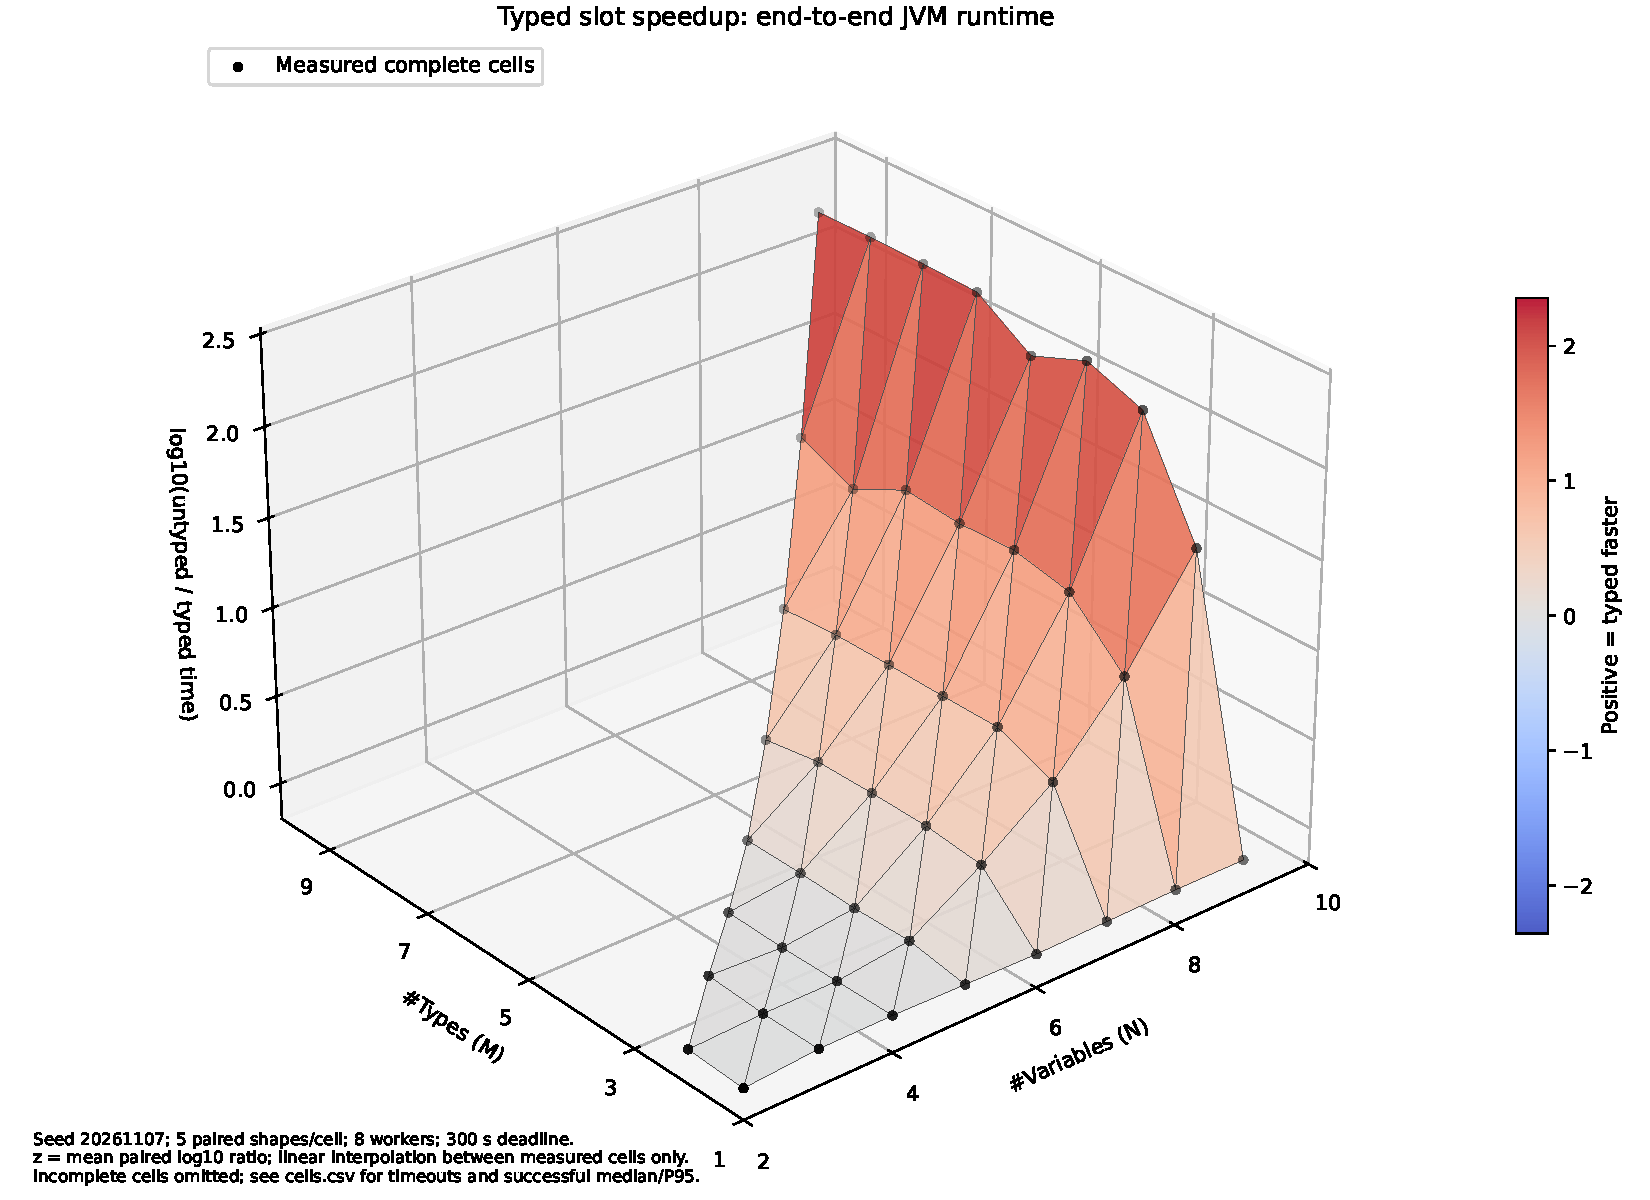
\includegraphics[width=0.78\linewidth]{figures/wall-speedup-surface.pdf}
\caption{Synthetic typed-versus-untyped end-to-end JVM speedup surface
($\log_{10}$ ratio across the 44/54 complete matched cells, without
interpolating across censored timeout cells). Complements
Figure~\ref{fig:synthetic-grid}.}
\label{fig:synthetic-wall-surface}
\end{figure}

\subsection{Bounded Semantic Validation Checks}

The natural checker evaluated 4,499 distinct zero
claims in the source models and found no counterexamples at the recorded
bounds. Each of the four deliberately invalid probes was refused by all
seven ablation arms. The capability study ran 29 bounded
sample checks across the generated families.

\subsection{Reproduction Identifiers}

\begingroup
\def\UrlBreaks{\do\-\do\_\do\/\do0\do1\do2\do3\do4\do5\do6\do7\do8\do9%
  \do\a\do\b\do\c\do\d\do\e\do\f}
\Urlmuskip=0mu plus 1mu\relax
The v3.3 experiment froze commit \path{d5c0c2a07504d53b13b28c61e9e64768c37eb984}.
It used 16 workers, an 8\,GiB heap cap, reward pool 100 and seed
\texttt{55520260811}. The following identifiers preserve the v3 synthetic
and historical study configuration.
\begin{itemize}
\item Experiment commit: \path{2d70f89ab67241cd071387ecedd3b2f432821921}.
\item Release commit (tag \texttt{v3}): \path{8770cb4b5f7133bad78058d9bc214f0ca36130d0}.
\item Natural corpus SHA-256 (66,080 files):
  \path{d6741fbf4c4a9b3714d012d068f84cc918052f1f55211bf4d0443b990736a689}.
\item Synthetic scaling dataset SHA-256 (270 pairs / 540 predicates):
  \path{c490b2bb1e6199f2ed221aa3f1b2d22b1da5dd8604341f305302c27a45de6b5f}.
\item Rule set: \texttt{canonical-equivalences-v3-explicit-laws};\\
  repair metric manifest ID:\\
  \texttt{certified-fast-rewrite-repair-distance-v25-}\\
  \texttt{retained-phase-representation}.
\item Natural and capability environment: AMD Ryzen~9 9950X3D (32 logical
  processors), OpenJDK~17.0.21.0.3, 16 workers, 8\,GiB heap, seed
  \texttt{55520260811}. Natural ablation run ID:
  \path{8dfc4fcc-84f0-4e9e-a88f-218fe05439b6}.
\item Synthetic grid environment: 8 concurrent isolated JVMs, 768\,MiB heap per
  JVM, 300-second deadline per predicate per arm; run ID:
  \path{e3d9bc4e-a514-471b-9e01-162562663f2e}.
\end{itemize}
\endgroup
